\subsection{Probabilistic payments}
In traditional payment channels, two parties A and B lock some funds within a smart contract, make multiple transactions off-chain and only commit the aggregation on-chain. By default a channel is bidirectional which means that both A and B can send and receive transactions within the channel no matter who created it. There is another type of channels which we use in HOPR called unidirectional channels where the channel creator is the sole owner of funds in the channel and the one able to create tickets. A channel created from A to B is different from a channel created from B to A.
 $$A\rightarrow B \neq B\rightarrow A$$
HOPR uses $acknowledgements$ which allow every node to create a message that acknowledges the processing of the packet to the previous node. This acknowledgement contains the cryptographic material to unlock the payout for the previous node. Note that acknowledgement is always sent to the previous node - even if there was no payment.
\\The fact that we are using payment channels implies that the last HOPR acknowledgement contains all previous incentives plus the incentive for the most recent interaction
\begin{align}  
value_(ACK_n) &=\sum_{i=1}^nfee_{packet_i}
     \end{align}
where $n$ is the total number of mixnet packets transformed.
\\~\\If B received $ACK_n$ for $packet_n$ before sending $packet_{n-1}$, it has no incentive to process $packet_{n-1}$ rather than $packet_{n}$.
\\~\\To avoid this limitation of traditional payment channels, HOPR utilizes probabilistic payments
\\~\\In probabilistic payments, the payouts use a concept called “tickets” (see section \nameref{ticket}), a ticket can be either a win or a loss with a certain winning probability. This means nodes are incentivized to continue relaying packets as they don’t know which ticket is a win.
\\~\\HOPR uses a custom-made layer 2 solution. It is inspired by payment channels and probabilistic payments where incentives can be claimed independently:
\begin{align}  
 value ( ACK_i )  &  =value ( ACK_j ) \quad for \quad i,j\in \{1,n\}
         \end{align}
Hence, there is no added value in pretending packet loss or intentionally changing the order in which packets are processed.
\subsubsection{Channel management}
Initially, each payment channel in HOPR is \textit{closed} which means that in order to transfer packets, those channels have to be opened. There are four distinct channel statuses which are represented in the following scheme:
\begin{figure}[H]
    \begin{center}
        

    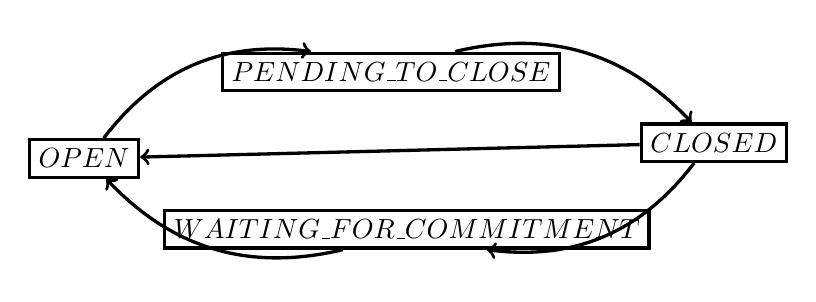
\begin{tikzpicture}
\begin{scope}[very thick,->]
    \path (-4,1)--(-4,0)--(0.1,0) node (commitment) [draw,align=left] {$WAITING\_FOR\_COMMITMENT$};
    \path  (0,0)--(4,0)--(4,1.1) node (closed) [draw] {$CLOSED$};
    \path (4,1)--(4,2)--(-0.1,2) node (pending) [draw,align=left] {$PENDING\_TO\_CLOSE$};
    \path (0,2)--(-4,2)--(-4,0.9) node (open) [draw] {$OPEN$};
    \draw [->,draw](closed) to [left] node {} (open);
    \draw [->,draw](commitment) to [bend left] node {} (open);
    \draw [->,draw](open) to [bend left] node [align=center] {} (pending);
    \draw [->,draw](pending) to [bend left] node {} (closed); 
    \draw [->,draw](closed) to [bend left] node {} (commitment); 


    
  \end{scope}
\end{tikzpicture}
\end{center}
\label{fig:channel statuses}
    \caption{Channel statuses}
\end{figure}
\paragraph{Opening a channel} Nodes can open channels to other nodes by the following:
A calls the method \textit{fundChannel()} or \textit{fundChannelMulti()}. The first function only funds the account of the sender (channel creator) and the second functions funds both accounts (sender and recipient). 
$$fundChannelMulti(A: <\lambda>, B:<\mu> )$$ where $\lambda$ and $\mu$ are the amounts to be staked by the sender (sender can be the same as A or B) for A and B. Both values can also be equal or any of them could be zero. The sender is also able to fund other channels which the sender is not part of.
Once the call has succeeded, an on-chain event \textit{WaitingForCommitment} is emited. 
\\~\\The destination address of the channel must now commit in order for the channel between both parties to be open. 
The channel destination (let's say it's B) can now call \textit{bumpChannel()} function to make a new set of commitments towards this channel. This call will trigger an onchain event \textit{ChannelIsOpened} and bumbs the ticket epoch to ensure tickets with the previous epoch are invalidated
\paragraph{Redeem tickets}
As long as the channel remains open, nodes can claim their incentives for forwarding packets which is represented as tickets (see ticket section). Tickets are redeemed by dispatching a \textit{redeemTicket()} call. The balance of the channel is then updated according to the balance defined in the ticket.
\paragraph{Closing a channel}
Nodes can close a payment channel in order to access their funds. The way to do so is using a timeout.
Only the channel creator (let's say it's A) can initiate the process by calling \textit{initiateChannelClosure()}. This changes the state to $pending\_timeout$ and triggers an on-chain event. Other nodes should monitor blockchain events to be aware of this change and thus will have now time to claim not yet claimed tickets. 
\\~\\Once the timeout is done, (A) can call \textit{finalizeChannelClosure()} which turns the channel state into \textit{closed}. When channel is closed, funds (stake) are transfered automatically back to (A). Every ticket that wasn't redeemed while channel was open can't be redeemed after closure.

\begin{comment}
    

\begin{figure}[H]
    \centering
    \begin{tikzpicture}[looseness=1,auto]
        \path (0,0) node (closed) [ellipse,draw] {$Closed$};
        \path (-1,-1)  node (commitment) [ellipse,draw,align=left] {$Waiting$\\$Commitment$};
        \path (5,0)  node (open) [ellipse,draw] {$Open$};
        \path (2.5,-1)  node (pending) [ellipse,draw,align=left] {$Pending$\\$Timeout$};

        \draw [->,draw](closed) to [bend left] node {\textsf{fund()}} (commitment);
        \draw [->,draw](commitment) to [bend left] node {\textsf{fund()}} (open);
        \draw [->,draw](open) to [bend left] node [align=center] {\textsf{initiateChannelClosure()}} (pending);
        \draw [->,draw](pending) to [bend left] node {\textsf{finalizeChannelClosure()}} (closed);

        \path[->] (open) edge [out=+120,in=+60,distance=2em,below] node [align=center,above] {\textsf{redeemTicket()}}  (open);
    \end{tikzpicture}
    \label{fig:channel workflow}
    \caption{Channel workflow}
\end{figure}
\end{comment}


\begin{comment}
  \draw [->,draw](commitment) to [bend left] node {\textsf{fund()}} (open);
    \draw [->,draw](open) to [bend left] node [align=center] {\textsf{initiateChannelClosure()}} (pending);
    \draw [->,draw](pending) to [bend left] node {\textsf{finalizeChannelClosure()}} (closed);  
\end{comment}

       
